%&latex
\documentclass[11pt,a4paper]{scrartcl}

\usepackage[english]{babel}
\usepackage{standalone}
\usepackage{layouts}
\usepackage{geometry}
 \geometry{
 a4paper,
 margin=20mm
 }
%\usepackage{showframe}

%--Fonts---%
\newcommand\hmmax{0} %Avoid too many alphabets error
\newcommand\bmmax{0}
\renewcommand{\rmdefault}{ppl} % rm
\linespread{1.05}        % Palatino needs more leading
\usepackage[scaled]{helvet} % ss
\usepackage{courier} % tt
\usepackage{mathpazo} 
\usepackage{microtype}

%---Encoding---%
\usepackage[utf8]{inputenc}
\usepackage[T1]{fontenc}
\usepackage{lmodern}
\usepackage{csquotes}
\usepackage[ddmmyyyy,hhmmss]{datetime} %Compilation date

%---Math---%
\usepackage{amsmath,amsthm,amstext,amsbsy,amsfonts,amssymb,stackengine}
\usepackage{mathrsfs}
\usepackage{cancel}
\usepackage{bm}
\usepackage{mathtools}
\usepackage{mathdots}
\usepackage{thmtools}
\usepackage{array}
\usepackage{yhmath}
\usepackage{gensymb}
\usepackage{blkarray}
\usepackage{xfrac}

%---Plots---%
\usepackage{epstopdf}
\usepackage{gnuplottex}
\usepackage{calc}
\usepackage{graphicx}
\usepackage{color}
\usepackage{transparent}

%---Physics---%
\usepackage{physics}
\usepackage{siunitx}
\sisetup{
separate-uncertainty = true
}

%---Tables---%
\usepackage{booktabs}
\usepackage{multirow}

\setlength{\aboverulesep}{0pt} %removes annoying spaces in booktabs tables
\setlength{\belowrulesep}{0pt}
\setlength{\extrarowheight}{.75ex}
\setlength\parindent{0pt} 

%---Graphics & Plots---%
\usepackage{color}
\usepackage[usenames, dvipsnames, table]{xcolor} %colori
\usepackage{wrapfig}
\usepackage[font=footnotesize, labelfont=bf,
            labelformat=parens,
            labelsep=endash, justification=raggedright,
            singlelinecheck=on]{caption} %fancy captions
\usepackage{subcaption} 
\usepackage{pgf,tikz}
\usetikzlibrary{arrows}
\usetikzlibrary{tikzmark}
\usetikzlibrary{patterns}
\usepackage{soul}
\usepackage[framemethod=tikz]{mdframed}
\usepackage{fancybox}
\usepackage{framed}

%---Indeces, links, bibliography---%
\usepackage{imakeidx} %Indice analitico
\usepackage[stable]{footmisc}

%\usepackage{xr-hyper}
\PassOptionsToPackage{hyphens}{url}\usepackage{hyperref}  %hyperref va caricato sempre dopo footmisc, altrimenti le footnotes si buggano e riportano tutte alla prima pagina
%\usepackage[inline]{showlabels} %Draft

\usepackage[symbol=$\wedge$,numberlinked=false]{footnotebackref}
\makeindex[columns=2, title=Analytical index, options= -s indexstyle.ist]

\usepackage[backend=biber,sorting=none]{biblatex}
\renewbibmacro{in:}{}
\addbibresource{bibliography.bib}

%---Utilities---%
\usepackage{comment}
\usepackage{xspace}
\usepackage{marginnote}
\usepackage{ragged2e}
\usepackage{enumerate}
\usepackage{enumitem}
\usepackage{etoolbox}
\usepackage{xargs}                      % Use more than one optional parameter in a new commands
\usepackage{lipsum}  
\usepackage{float}

\usepackage{lipsum}  
\usepackage{float}
\usepackage{listings}
\usepackage[most]{tcolorbox}

\newcommand{\opx}[1]{\hat{\mathrm{#1}}}
\newcommand{\bb}[1]{\mathbb{#1}}

%%%%%%%%%% CODE LISTING %%%%%%%%%%%
%New colors 
\definecolor{codegreen}{rgb}{0,0.6,0}
\definecolor{codegray}{rgb}{0.5,0.5,0.5}
\definecolor{codepurple}{rgb}{0.58,0,0.82}
\definecolor{backcolour}{rgb}{0.95,0.95,0.92}
%Code listing style named "mystyle"
\lstdefinestyle{mystyle}{
  language=[90]Fortran,
  backgroundcolor=\color{backcolour},   commentstyle=\color{codegreen},
  keywordstyle=\color{magenta},
  numberstyle=\tiny\color{codegray},
  stringstyle=\color{codepurple},
  basicstyle=\ttfamily\footnotesize,
  breakatwhitespace=false,         
  breaklines=true,                 
  captionpos=b,                    
  keepspaces=true,                 
  numbers=left,                    
  numbersep=5pt,                  
  showspaces=false,                
  showstringspaces=false,
  showtabs=false,                  
  tabsize=2
}
%"mystyle" code listing set
\lstset{style=mystyle}

\usepackage{fancyhdr}
\pagestyle{fancy}
\fancyhf{} %Clear the previous header/footer

\lhead{Francesco Manzali}
\rhead{\today}
\lfoot{Neural Networks and Deep Learning A.A. 2020/21}
\rfoot{Assignment \exerciseNumber, page \thepage}

\newcommand{\exerciseNumber}{2}
\newcommand{\q}[1]{``#1''} 
\setlength{\parskip}{0cm}

\graphicspath{{Plots/}}
\begin{document}

%+Title
\title{Unsupervised Deep Learning}
\subtitle{Assignment \exerciseNumber}
\author{\large Francesco Manzali}
\date{\large \today}
\maketitle
\thispagestyle{fancy}
%-Title

%+Abstract
\begin{abstract}
  In unsupervised learning, useful features are learned directly from data, without the need of any labels. Autoencoders are a common neural network architecture for solving such problem. This homework explores different kinds of autoencoders, evaluating their performance through their reconstruction error, and inspecting their learned latent spaces. Moreover, autoencoders are shown to be useful for training supervised models more quickly. 
\end{abstract}
%-Abstract


%Total length <= 6 pages, additional tables/figures can be added in a final appendix (optional)

\section*{Introduction}
An \textbf{autoencoder} is a type of neural network constructed to learn latent representations of unlabeled data. It consists of two parts:
\begin{itemize}
    \item An \textit{encoder}, which maps input samples to their latent representations
    \item A \textit{decoder}, which (approximately) reverses the encoder mapping.
\end{itemize}
The main idea is that the network tries to store all the \q{relevant} information about the inputs in the latent space, so that it can be reconstructed by the decoder. The difference between an input and the reconstruction of its representation is quantified by the \textit{reconstruction error}, which is minimized during training. 

\medskip

In this homework, autoencoders are trained on the MNIST dataset of digits, which is split into $\num{48000}$ samples for training, $\num{12000}$ for validation and the remaining $\num{10000}$ for the final testing. 

\medskip

In sec.~\ref{sec:cnn_autoencoder} a first convolutional autoencoder is tested, and its hyperparameters are optimized. Then, sec.~\ref{sec:cnn_denoiser} tests the same architecture on the task of reconstructing noisy samples. Sec.~\ref{sec:vae} presents a variational autoencoder, which is regularized to learn more interpretable representations. Finally, sec.~\ref{sec:supervised} shows how a pretrained autoencoder can help the construction of a small supervised network, which is able to quickly reach a good performance.

\medskip

All networks are implemented using the PyTorch Lightning library \cite{pytorch_lightning}, while Optuna \cite{optuna} is used for the hyperparameters search. 


%Homework goals and the main implementation strategies chosen

\section{Convolutional Autoencoder \label{sec:cnn_autoencoder}}
\subsection{Methods}
The architectures for the encoder and decoder are shown in fig.~\ref{fig:cnn_architecture}. They consist of a $3$-layer convolutional segment, followed by $2$ fully connected layers, and they exactly mirror each other. 

The ReLU activation is used for all hidden layers, since it helps avoiding the gradient vanishing problem. The encoder's output has no activation, while a sigmoid is applied after the decoder's output, since the dataset is normalized to have values in $[0,1]$. Dropout is applied after each hidden layer, both in the convolutional and fully-connected segments. MSE is always used as the loss function.

\medskip

The search space for hyperparameters, and the final values found by optimization through Optuna are shown in tab.~\ref{tab:hyperparameters} (a complete log can be found in the Appendix, in fig.~\ref{fig:cnn_hyperparameters}).
They are used for all subsequent models, if not specified otherwise. Notably, the optimal latent space is not the highest allowed, meaning that few dimensions suffice to capture all the data variability. 

\begin{table}[H]
    \centering
    \begin{tabular}{@{}cccccc@{}}
    \toprule
    \multicolumn{1}{l}{} &
      \textbf{Dim. Latent Space} &
      \textbf{Optimizer} &
      \textbf{Learning rate} &
      \textbf{Batch size} &
      \textbf{Dropout} \\ \midrule
    \textbf{Search} &
      \begin{tabular}[c]{@{}c@{}}$[2, 50]$\\ (uniform)\end{tabular} &
      Adam or SGD &
      \begin{tabular}[c]{@{}c@{}}$[10^{-5}, 10^{-2}]$\\ (log-uniform)\end{tabular} &
      $64$, $128$, $256$ &
      \begin{tabular}[c]{@{}c@{}}$[0, 1]$\\ (uniform)\end{tabular} \\
    \textbf{\begin{tabular}[c]{@{}c@{}}Best\\ (100 trials)\end{tabular}} &
      $33$ &
      Adam &
      $\num{5.4e-3}$ &
      $128$ &
      $\num{1.2e-2}$ \\ \bottomrule
    \end{tabular}
    \caption{Hyperparameters for the convolutional autoencoder.}
    \label{tab:hyperparameters}
\end{table}

\begin{figure}[H]
    \centering
    \begin{subfigure}[t]{0.9\textwidth}
        \centering
        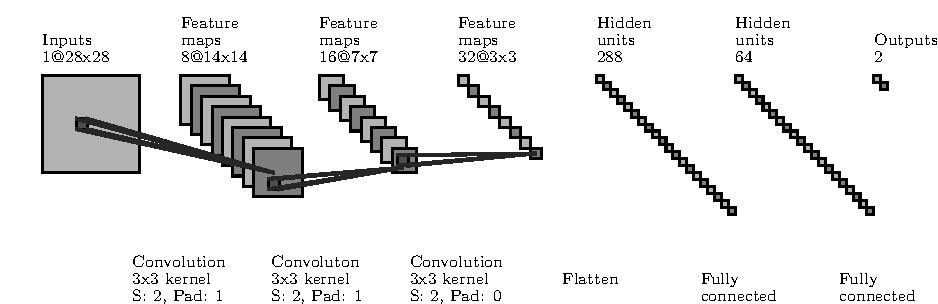
\includegraphics[width=\textwidth]{Images/encoder_fig}
        \caption{Encoder architecture}
    \end{subfigure}\\

    \begin{subfigure}[t]{0.9\textwidth}
        \centering
        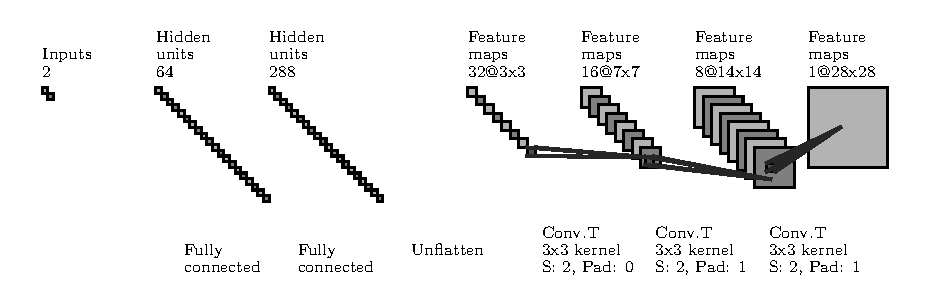
\includegraphics[width=\textwidth]{Images/decoder_fig}
        \caption{Decoder architecture}
    \end{subfigure}%
    \caption{Architecture of the convolutional autoencoder. The size of the encoder output (equal to that of the decoder input) is the dimension of the latent space ($2$ in the figure). \label{fig:cnn_architecture}}
\end{figure}


\subsection{Results}
The autoencoder is then trained for $50$ epochs, using the best hyperparameters found and early stopping. The final MSE loss on the test dataset is $0.0087$, which is very good for this dataset. Some examples of reconstruction from the validation set are shown in fig.~\ref{fig:samples_cnn}, and are all satisfactory. 

\medskip

A few more pictures are available in the Appendix. First, the learning curves for the reconstruction error are shown in fig.~\ref{fig:best_learning_curve}. Fig.~\ref{fig:best_pca} and \ref{fig:best_tSNE} show the PCA/t-SNE projection of latent representations of digits. From these, especially the latter, it can be seen that the model learns to cluster together images of the same digit, even if it is not provided any label for them. Finally, an autoencoder is trained with a $2d$ latent space, which allows to directly plot the representations as points in a plane (fig.~\ref{fig:2d_encoded_space}). 

\begin{figure}[H]
    \centering
    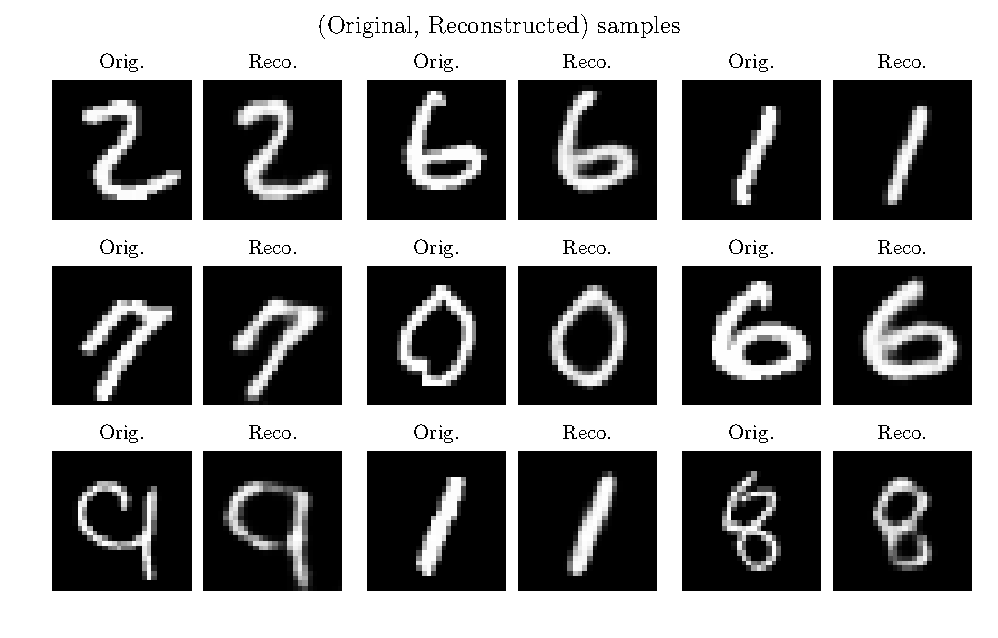
\includegraphics[width=\textwidth]{../Code/Plots/orig_reconstructed}
    \caption{Samples reconstructed by the CNN autoencoder.\label{fig:samples_cnn}}
\end{figure}

\section{Denoising Autoencoder\label{sec:cnn_denoiser}}
\subsection{Methods}
In this application, samples are shown to the convolutional autoencoder with added noise (fig.~\ref{fig:noise_types}). The architecture is the same described in the previous section, and the reconstruction error still measures the distance between the reconstructed digits and the original ones, without noise. This means that, effectively, the model is trained to \textit{remove} the noise from the input samples.

\begin{figure}[H]
    \centering
    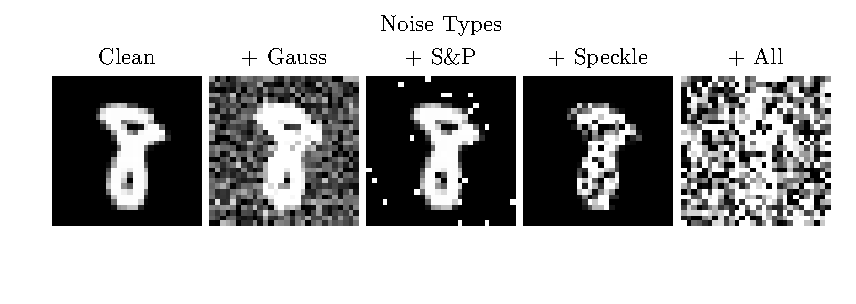
\includegraphics[width=0.8\textwidth]{../Code/Plots/noise_types}
    \vspace{-2em}
    \caption{Types of noise considered for generating the training samples. \textbf{Gaussian}: random samples from a normal distribution $\mathcal{N}(0.5, 0.3)$ are added to the image. \textbf{Salt \& Pepper} (S\&P): one out of $20$ pixels is set to $1$ (salt) or $0$ (pepper) with equal probability. \textbf{Speckle}: a random filter is constructed by sampling a gaussian $\mathcal{N}(0, .5)$. Then the image is multiplied by the filter, and the result is added to the original image. In all cases, pixel values are clipped between $0$ and $1$ after applying the noise. \label{fig:noise_types}}
\end{figure}

\subsection{Results}
Training for $50$ epochs with the same hyperparameters from tab.~\ref{tab:hyperparameters} allows to reach a test MSE loss of just $0.03$. The added noise has clearly made reconstruction much more difficult (fig.~\ref{fig:samples_denoising}), and some digits are not correctly retrieved. Nonetheless, the model is powerful enough to resolve an amount of noise that is challenging even for humans, which is remarkable.

\begin{figure}[H]
    \centering
    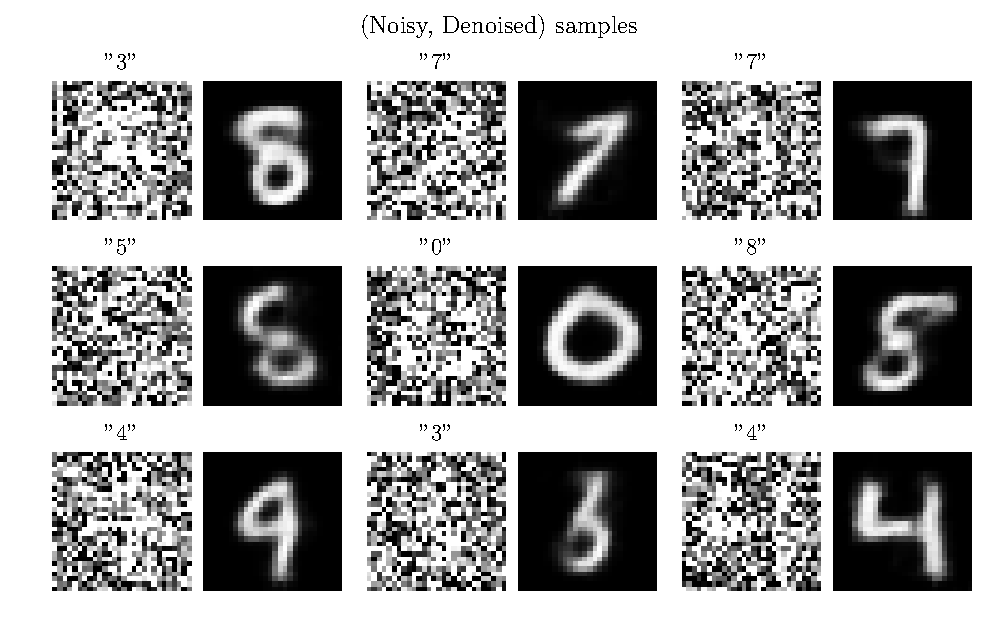
\includegraphics[width=\textwidth]{../Code/Plots/noisy_denoised}
    \caption{Samples reconstructed by the denoising autoencoder.\label{fig:samples_denoising}}
\end{figure}

\section{Variational Autoencoder\label{sec:vae}}
Variational autoencoders use an entirely different process for reconstructing images. In fact, in this case the \textit{encoder} does not output directly a latent vector, but rather the parameters of a probability distribution from which the latent vector can be sampled. The ability to choose that distribution, and to force it to be the \q{simplest} possible through regularization, allows to obtain an unsupervised learner that is more robust to noise, and learns more interpretable representations.

\subsection{Methods}
The \textit{encoder} architecture from fig.~\ref{fig:cnn_architecture} is changed to output the parameters of a multivariate Normal distribution $\mathcal{N}(\bm{\mu}, \Sigma)$ with diagonal covariance matrix $\Sigma = \operatorname{diag}(\sigma_1^2, \dots, \sigma_d^2)$, chosen for its simplicity and efficiency. Specifically, the convolutional segment is kept unchanged, but its output is sent to two independent copies of the fully-connected segment: one computes the entries of the mean vector $\bm{\mu} = (\mu_1, \dots, \mu_d)^T$, while the other returns the logarithm of the variances $(\log \sigma_1^2, \dots, \log \sigma_d^2)^T$. In this way, a sample $\bm{s}$ can be generated as follows:     
\begin{align*}
    \bm{s} = \bm{\mu} + \bm{\xi} \odot \exp(\frac{1}{2} \log \bm{\sigma}^2) = \bm{\mu} + \bm{\xi} \odot \bm{\sigma} \qquad \bm{\xi} \sim \mathcal{N}(\bm{0}, \bb{1}_d)
\end{align*}
where all operations, such as exponentiation ($\bm{\sigma}^2$) or multiplication ($\odot$) are element-wise. Note that the randomness is completely contained in the separate $\bm{\xi}$ factor, and that the expected value of $\bm{s}$ is differentiable with respect to the network's parameters used to compute $\bm{\mu}$ and $\bm{\sigma}$, allowing to apply backpropagation.

\medskip

The loss function, taken from \cite{vae}, consists of a reconstruction error term (MSE) and a regularization term, which forces the learned distribution to be as close as possible to a standard Normal distribution $\mathcal{N}(\bm{0}, \bb{1}_d)$:
\begin{align*}
    \mathcal{L}(\bm{x}, \hat{\bm{x}}) = \norm{\bm{x} - \hat{\bm{x}}}^2 + \mathrm{KL}[\mathcal{N}(\bm{\mu}, \Sigma), \mathcal{N}(\bm{0}, \bb{1}_d)] =  \norm{\bm{x} - \hat{\bm{x}}}^2 - \frac{1}{2} \sum_{j=1}^d (1 + \log (\sigma_j^2) - \mu_j^2 - \sigma_j^2) 
\end{align*}
where $\bm{x}$ denotes an input sample, $\hat{\bm{x}}$ is the reconstructed sample by the decoder, and $\mathrm{KL}$ is the Kullback-Leibler divergence, measuring the distance between two probability distributions. 

\subsection{Results}
The network is trained for $100$ networks, with no dropout, Adam as optimizer with $\lambda=10^{-3}$ and a latent space of dimension $33$. Overfitting is mitigated by stopping training if the validation loss has not decreased for $10$ epochs. 

A few reconstructed samples are shown in fig.~\ref{fig:samples_vae}. The quality is a bit lower than that of the convolutional autoencoder from sec.~\ref{sec:cnn_autoencoder}, due to the much more significant regularization. 

However, the final representations are more robust: a small change in the input is mapped to a small change in the latent space. This nice property allows to compute \q{transitions} between images, by starting from a representation vector and moving step by step along the line that connects it to some other target vector. This is shown in fig.~\ref{fig:vae_transition}, where a \q{$0$} is gradually transformed to a \q{$9$}. Interestingly, the middle image looks like a \q{$8$}, which is intuitively an intermediate shape between the two digits.


\begin{figure}[htp]
    \centering
    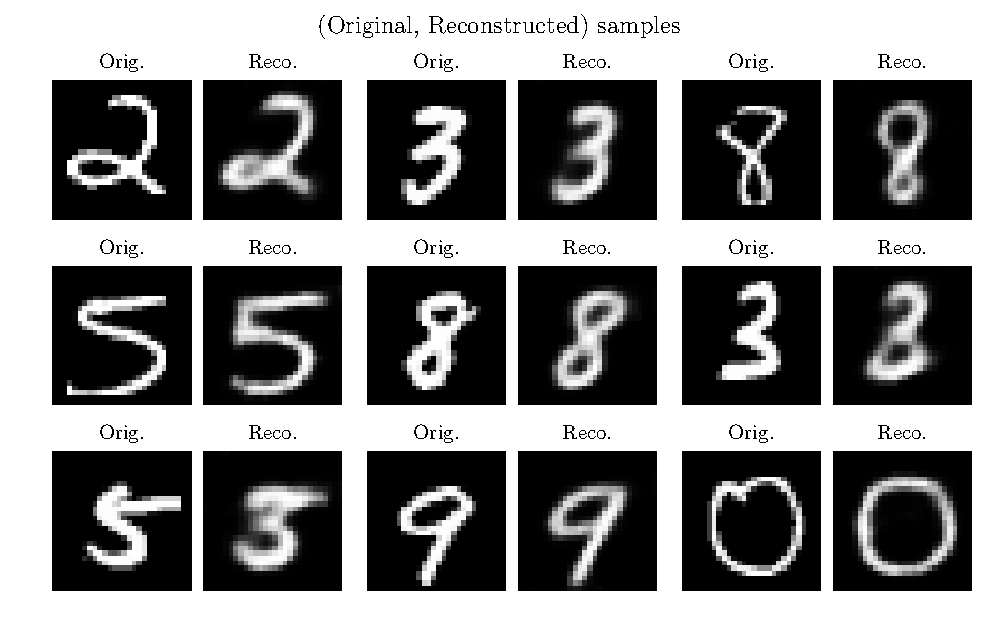
\includegraphics[width=\textwidth]{../Code/Plots/orig_reconstructed_vae}
    \caption{Samples reconstructed by the variational autoencoeder.\label{fig:samples_vae}}
\end{figure}

\begin{figure}[htp]
    \centering
    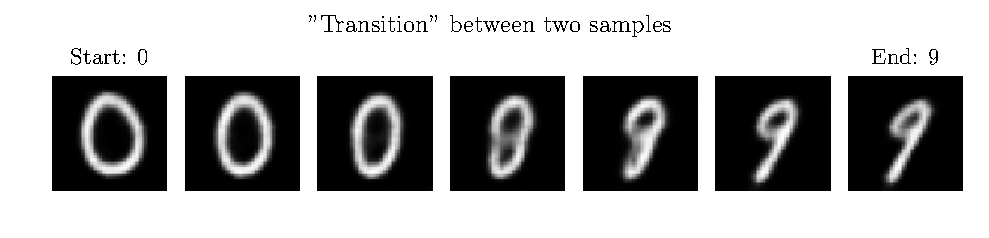
\includegraphics[width=\textwidth]{../Code/Plots/vae_transition}
    \caption{In a variational autoencoder, a linear interpolation between two latent representations produces a \q{smooth} transition between the digits they represent.\label{fig:vae_transition}}
\end{figure}

In the appendix, the latent representations from a $2d$ variational autoencoder are directly plotted (fig.~\ref{fig:2d_encoded_space_vae}), so that they can be compared with those from a normal convolutional autoencoder (fig.~\ref{fig:2d_encoded_space}). Note how, in the variational case, clusters are more well separated and \q{regular}.

\section{Transfer Learning\label{sec:supervised}}
A pretrained autoencoder can be \textit{fine-tuned} to a supervised task, such as classification, significantly speeding up the training process, while reaching comparable results to end-to-end training.

\subsection{Methods}
To test this, the \textit{encoder} part of the convolutional autoencoder from sec.~\ref{sec:cnn_autoencoder} is \q{attached} to just two fully-connected layers with $128$ and $10$ neurons each, separated by a ReLU activation. Then, only the parameters of the latter segment are trained, while keeping all the ones from the encoder fixed to their previously learned values. 


\subsection{Results}
The final network is trained for $50$ epochs with early stopping, Adam with $\lambda = \num{5e-3}$ and no regularization. The loss converges after just $22$ epochs, with a final train accuracy of $99\%$, and $98.1\%$ on both the validation and the test datasets. This performance is good for such few trainable parameters (less than $6$k), and training is very fast, requiring just a few minutes. Note also that no hyperparameter finetuning was done. 

However, the best network from the first homework reached a $99.5\%$ accuracy on the test dataset, albeit requiring a full $100$ epochs and an extensive grid search for the hyperparameters. Thus, exploiting a pretrained network is good for reaching acceptable results quickly, but getting the best possible score requires a full training procedure. 

\medskip
The learning curve for this supervised task is shown in fig.~\ref{fig:supervised_learning_curves} in the Appendix.

\printbibliography
\clearpage

\section*{Appendix}

\begin{figure}[H]
    \centering
    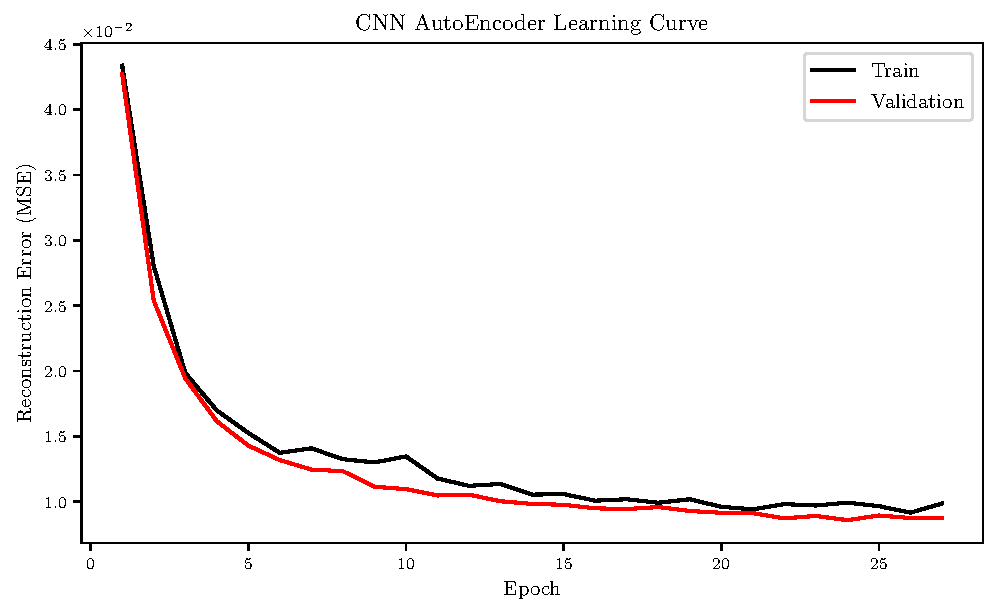
\includegraphics[width=.9\textwidth]{../Code/Plots/best_hyperparams_learning_curve}
    \caption{Learning curves for the CNN Autoencoder with the best hyperparameters found.\label{fig:best_learning_curve}}
\end{figure}

\begin{figure}[H]
    \centering
    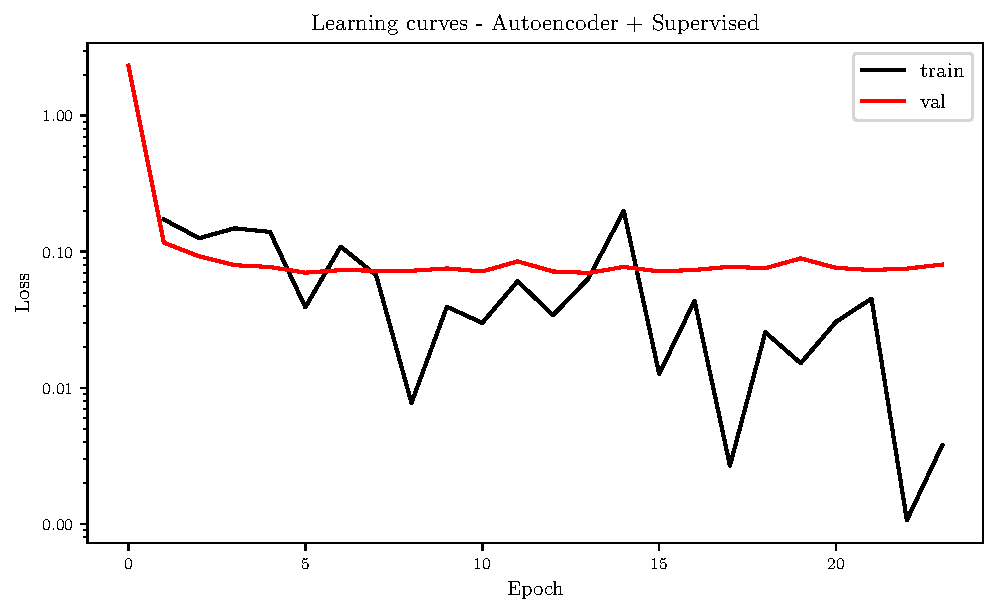
\includegraphics[width=.9\textwidth]{../Code/Plots/learning_curves_supervised}
    \caption{Learning curves for the supervised classfier trained on top of a pretrained CNN autoencoder.\label{fig:supervised_learning_curves}}
\end{figure}

\begin{figure}[htp]
    \centering
    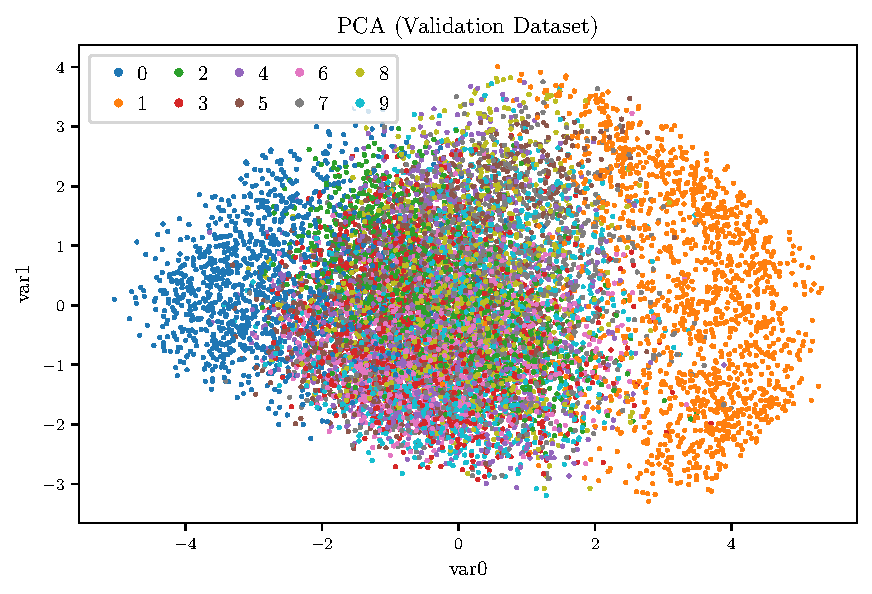
\includegraphics[width=.9\textwidth]{../Code/Plots/best_hyperparams_PCA}
    \caption{PCA projection of the latent representations of MNIST digits from the validation set, as learned by the CNN Autoencoder (best hyperparameters).\label{fig:best_pca}}
\end{figure}

\begin{figure}[htp]
    \centering
    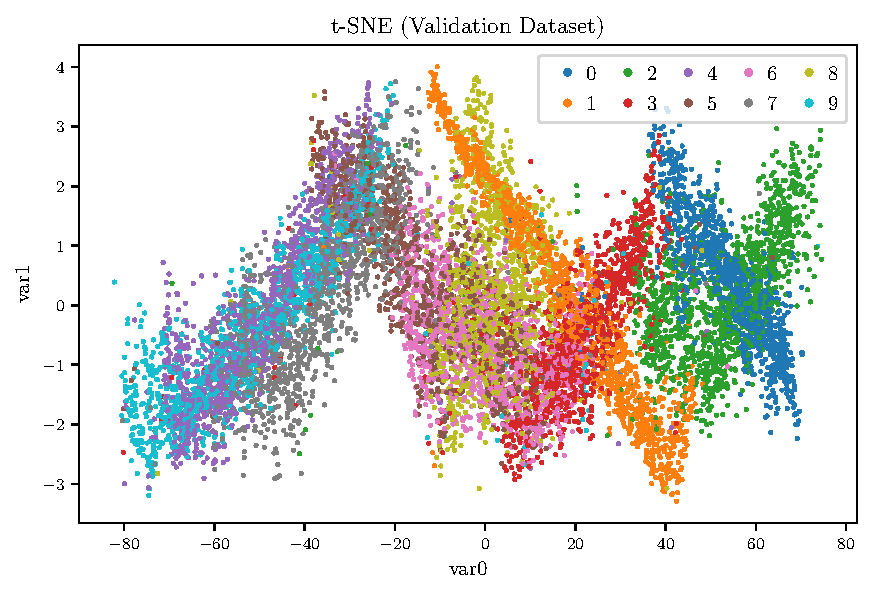
\includegraphics[width=.9\textwidth]{../Code/Plots/best_hyperparams_tSNE}
    \caption{t-SNE projection of the latent representations of MNIST digits from the validation set, as learned by the CNN Autoencoder (best hyperparameters).\label{fig:best_tSNE}}
\end{figure}

\begin{figure}[htp]
    \centering
    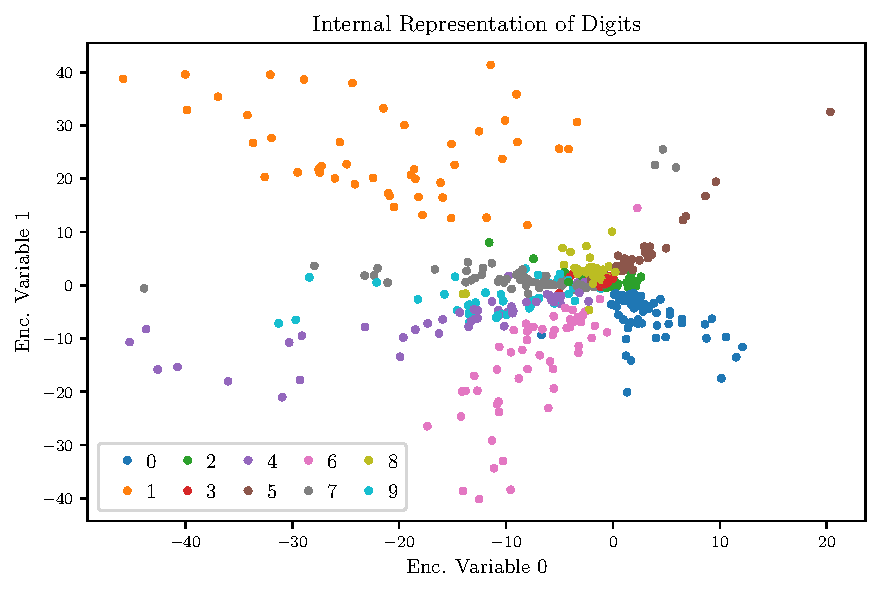
\includegraphics[width=.9\textwidth]{../Code/Plots/2d_encoded_space}
    \caption{Direct plot of a few latent representations from a CNN autoencoder with a 2D latent space. Note that images of the same digit form recognizable clusters, meaning that the network is able to learn which images are representing the \textit{same} digit.\label{fig:2d_encoded_space}}
\end{figure}

\begin{figure}[htp]
    \centering
    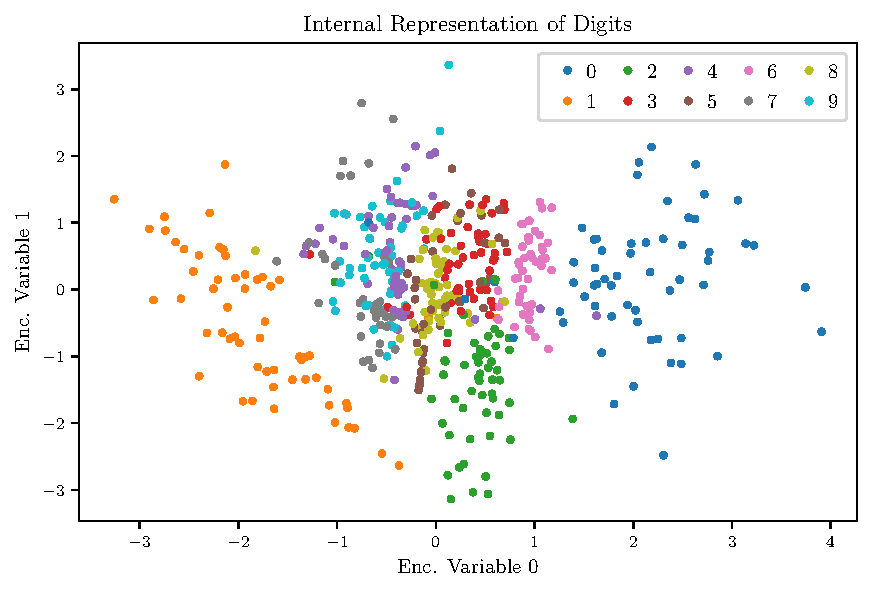
\includegraphics[width=.9\textwidth]{../Code/Plots/2d_encoded_space_vae}
    \caption{Direct plot of a few latent representations from a variational autoencoder with a 2D latent space. Note how clusters are more \q{sparse}, and how digits that are visually similar (e.g. $8$ and $9$) are close together.\label{fig:2d_encoded_space_vae}}
\end{figure}

\begin{figure}[htp]
    \centering
    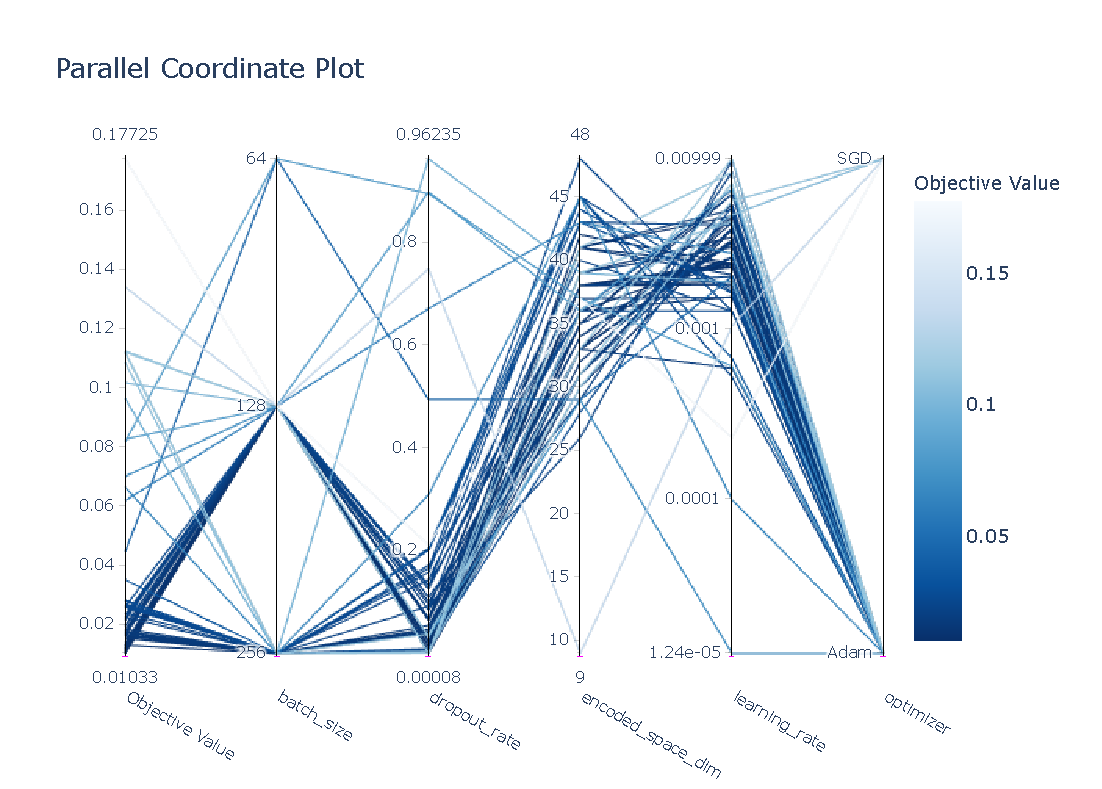
\includegraphics[width=\textwidth]{../Code/Plots/hyperparameters}
    \caption{Log of the hyperparameters search for the CNN autoencoder.\label{fig:cnn_hyperparameters}}
\end{figure}

%All pictures should have a reference [OK]

%\the\textwidth


\end{document}
